\documentclass[12pt, letterpaper]{elsarticle}
\usepackage[utf8]{inputenc}
\usepackage{graphicx}
\usepackage{siunitx}

\title{Neutronics aspects of the FESS-FNSF}
\author[wisc]{A. Davis\corref{cor1}}
\ead{andrew.davis@wisc.edu}
\author[wisc]{M. Harb}
\ead{mharb@wisc.edu}
\author[wisc]{L. El-Guebaly}
\ead{elguebaly@wisc.edu}
\author[wisc]{P. Wilson}
\ead{paul.wilson@wisc.edu}
\author[wisc]{E. Marriott}
\ead{marriott@wisc.edu}
\ead[url]{http://cnerg.wisc.edu}
\cortext[cor1]{Corresponding author}

\address[wisc]{1500 Engineering Drive, Madison, WI 53706}
 
\begin{document}
 
\begin{abstract}
Neutronics analysis was performed on the latest Fusion Energy System Studies - Fusion Neutron Science Facility (FESS-FNSF) design which covered the neutron wall loading, tritium breeding ratio, radiation damage, and shutdown dose rate calculations. Sixteen different sector configurations were investigated with a main focus on determining the impact which each has upon the tritium breeding ratio (TBR) of the whole facility. This paper describes the stages of the nuclear analysis that serve to prove the radiation derived attributes of the system.

\vspace{5mm}
\noindent
Keywords: FESS-FNSF, tritium breeding ratio, radiation damage, shutdown dose rate, DAGMC
\end{abstract}

\begin{titlepage}
\maketitle
\end{titlepage}

\newpage
\listoffigures

\newpage
\section{Introduction} \label{Introduction}
The Fusion Energy Systems Studies - Fusion Nuclear Science Facility (FESS-FNSF \cite{ref_1}) is considered an essential element of the US fusion roadmap that displays a strategic  pathway from ITER, to US DEMO, and eventually to the first commercial power plant. A FNSF will help bridge the research gap between ITER - low radiation damage, short pulses, no tritium breeding - and DEMO which is designed to operate at power plant relevant fusion parameters. The FNSF will advance the understanding of fusion nuclear sciences (FNS) by providing an integrated platform for establishing a database on all components up to relevant parameters (e.g. 40-60 dpa, blanket temperatures 500-600\textsuperscript{o}C) via in-depth investigation of issues related to Plasma boundary interface (materials interaction with high energy neutron flux, surface/volumetric heating, radiation damage, and gas production), operating in power plant relevant fusion core conditions (temperatures, coolant/breeder flow rates, pressures/stresses, B-field, and neutrons), tritium breeding/extraction/processing, advancing and demonstrating plasma technologies that support very long duration operations, etc.\vspace{5mm}

The FNSF subjected to this study is a tokamak-based facility with a \SI{518}{MW} fusion power with a plant Lifetime $\sim$ \SI{24}{years} ($\sim$ \SI{8.5}{FPY}) and $\sim 35\%$ availability. The machine average neutron wall loading (NWL) is \SI{1.1}{MW/m\textsuperscript{2}}. The radiation damage to the first wall was calculated followed by a shielding analysis. Shielding optimization \cite{ref_2} involved testing the effect of the inboard shielding materials on the radiation damage levels at the magnet with an inboard breeding blanket and the results showed that the radiation levels at the magnet are within acceptable limits. Such calculations involved estimating the fast neutron fluence, nuclear heating at the coil case, and atomic displacement to the Cu stabilizer.\vspace{5mm}

A detailed tritium breeding study was also performed to assess the effect of various design elements on the tritium breeding ratio (TBR) of the dual-cooled lithium lead (DCLL) blanket which confirmed tritium self-sufficiency, a value of TBR $\sim$ 1 with 4\% margin. Following the TBR calculations, shutdown dose rate analysis was performed which involved irradiation of one sector in the model (without any penetrations or ports) and the operation of the facilty was assumed to be at constant flux levels for \SI{4.2}{years} followed by a complete shutdown. The dose rate was estimated at \SI{0}{s}, \SI{1}{d}, \SI{7}{d}, \SI{15}{d}, \SI{1}{y} following the shutdown.\vspace{5mm}

In section (\ref{Analysis Tools}) the software tools used in this study will be described and in section (\ref{Neutron Wall Loading}) NWL results will be introduced. In section (\ref{Tritium Breeding Calculations}) focus will be on the tritium breeding calculations. In section (\ref{Radiation Damage}) magnet shielding and radiation damage calculations will be discussed and finally in section (\ref{Shutdown Dose Rate Calculations}) the shutdown dose rate calculations will be presented.

\subsection{Configuration} \label{Configuration}
The first step in the analysis involved optimization of the OB and IB radial build and the divertor vertical build \cite{ref_2} and resulted in a complete definition of the material composition of the different regions taking into account the configuration of the facility, radiation limits especially at the magnet (and other long lifetime components), selection of low activation materials, environmental and safety constraints, and temperature limits for several in-vessel components. The OB radial build and the corresponding material composition of each layer is shown in figure \ref{fig:OB_radial} and the detailed composition is;
\begin{figure}[h!]
  \centering
  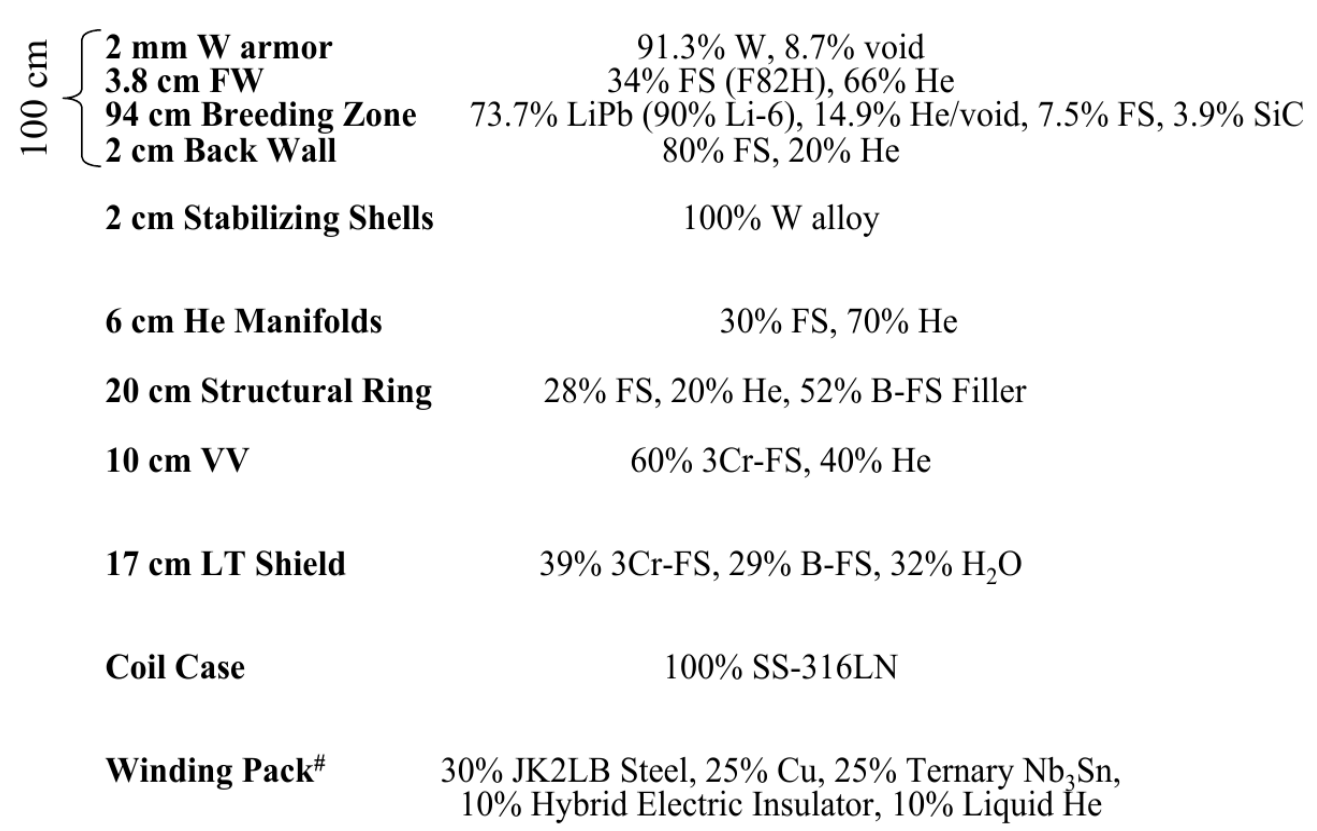
\includegraphics[scale=0.2]{../plots/OB_comp.png}
  \label{fig:OB_comp}
\end{figure}
\begin{figure}[h!]
  \centering
  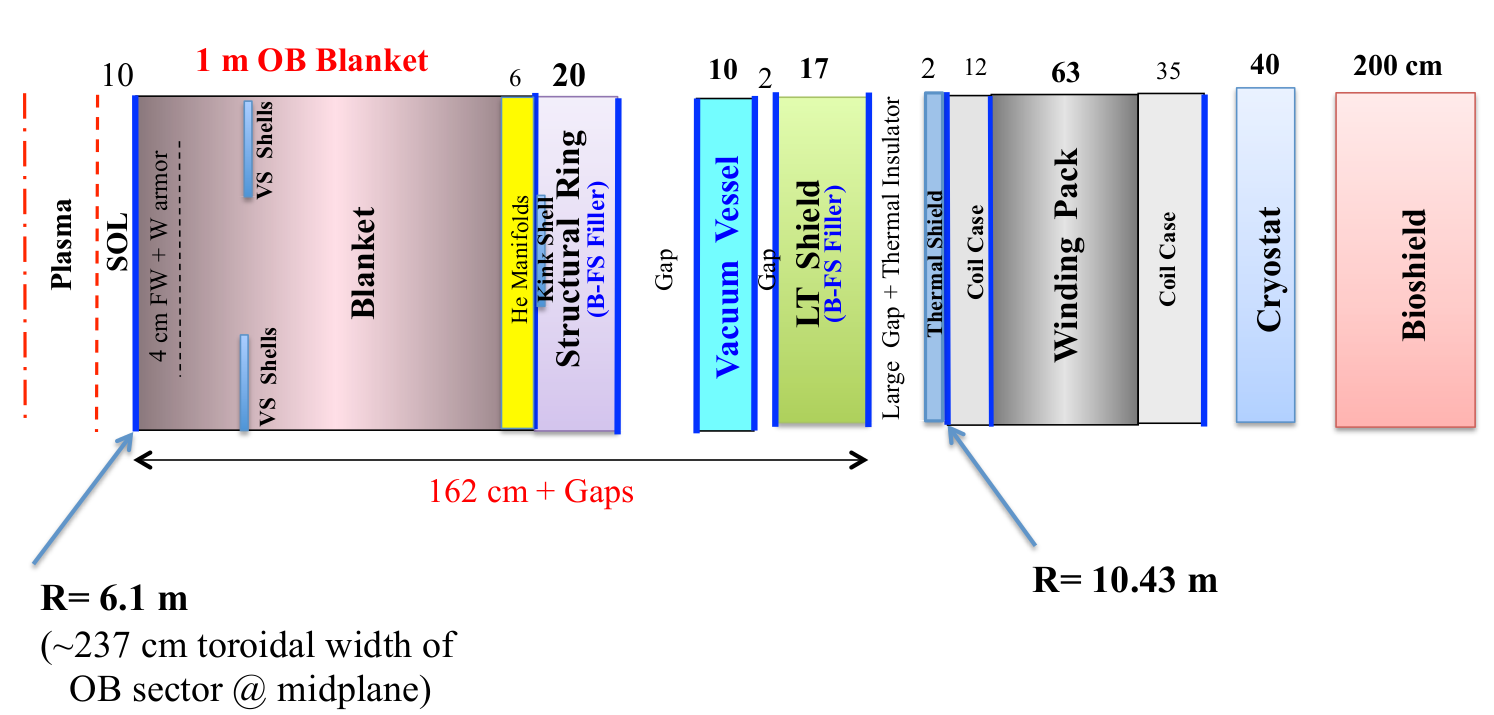
\includegraphics[scale=0.2]{../plots/OB_radial.png}
  \caption{The OB radial build}
  \label{fig:OB_radial}
\end{figure}

\subsection{Full 3D Build} \label{Full 3D Build}
The shielding and blanket optimization described in subsection (\ref{Configuration}) resulted in a full definition of the major materials and dimensions that were used to produced the 3D assembly CAD model. Shown in Figure \ref{fig:Full3D} is a cross section of one sector with the major regions identified on the figure. The model consists of 16 IB and OB sectors with 2 cm assembly gaps. The facility has a major Radius of \SI{4.8}{m} and a minor Radius of \SI{1.2}{m}.
\begin{figure}[h!]
  \centering
  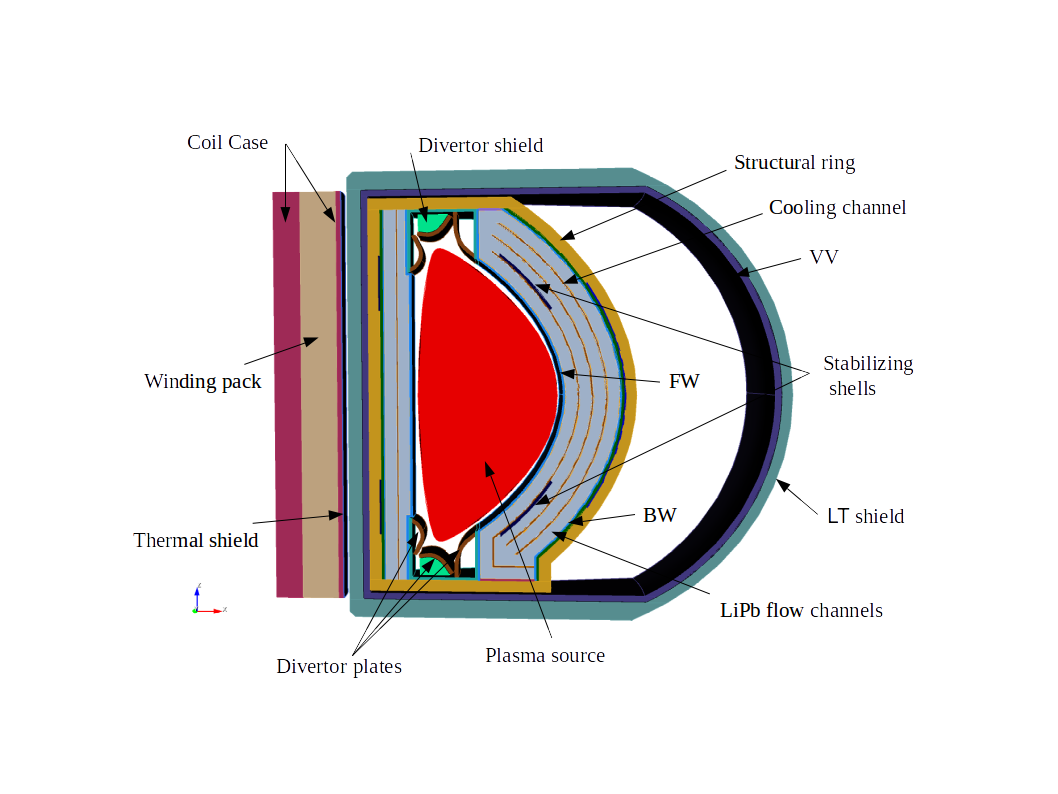
\includegraphics[scale=0.35]{../plots/full_3d.png}
  \caption{The full 3D CAD model of a single FESS-FNSF sector}
  \label{fig:Full3D}
\end{figure}

\section{Analysis Tools} \label{Analysis Tools}
As will be discussed in section (\ref{Tritium Breeding Calculations}), calculation of the TBR with high fidelity has to be achieved in order to confirm the adequacy of the configuration of the facility for tritium self-sufficiency. Based on previous analyses with similar models, some margins are considered in the design phase such that the final integration of all engineering systems in the facility will ensure a TBR $>$ 1. one of the margins \cite{ref_4} considered in the design phase of the facility is directly related to deficiencies in modelling resulting from approximations introduced to facilitate the analysis especially the neutron/photon transport calculations. In this study the approximations were applied to design details which are known – based on accumulated experience with previous models - to be of less importance regarding neutron/photon transport calculations besides slowing down the simulations if included. Such design details include; the detailed structure of the first wall “FW” and its He cooling system, the internal structure of the blanket cooling channels, and the internal structure of the He manifolds. Those regions are known to show little/no difference if modelled in detail or homogenized as one region with a proper assignment of volume averaged material compositions.\vspace{5mm}

State-of-the-art analysis tools were utilized in this study which enabled working with the full 3-D model with all the internal details defined in the CAD, such as blanket internals and side/back/front walls, which are known to play a key role in TBR degradation. This work was performed with DAG-MCNP5, a version of MCNP5 \cite{ref_5} that has been enhanced by the DAGMC \cite{ref_6} toolkit. Coupled with MCNP5, DAGMC provides remarkable capabilities for the analysis of complex fusion facilities by utilizing acceleration techniques to achieve efficient ray tracing directly on CAD solid models without the need to translate the geometry/model to the native input representation of the transport code. Other software tools were used for mesh representation of the geometry and application of transport variance reduction techniques for deep penetration in regions behind the shields and the fusion evaluated nuclear data library (FENDL2.1)\cite{ref_7} was used in this analysis. Utilization of such sophisticated tools allowed reducing the approximations involved in the analysis by incorporating fine details which previously represented a challenge. 

\subsection{Neutron Source Modelling} \label{Neutron Source Modelling}
An MCNP sampling routine was written to sample the neutrons for the transport calculations compared to the previous workflow which utilized either an approximated 3-region or R-Z sources. The physical parameters defining the plasma source \cite{ref_3} are: fusion power = 518 MW, major radius = 4.8 m, minor radius = 1.2 m, elongation = 2.2, triangularity = 0.625, Shafranov shift = 0.144 m, ion density in the pedistal, seperatrix, and core regions = 1x10\textsuperscript{20}/m\textsuperscript{3}, 0.56x10\textsuperscript{20}/m\textsuperscript{3}, and 1.6x10\textsuperscript{20}/m\textsuperscript{3} respectively with a peaking factor of 1.52 (peak to volume average), ion temperature in the pedistal, seperatrix, and core regions  = 4 keV, 100 eV, and 22 keV respectively with a peaking factor of 2.25 (peak to volume average), and pedistal radius = 1.14 m.
\begin{figure}[h!]
  \centering
  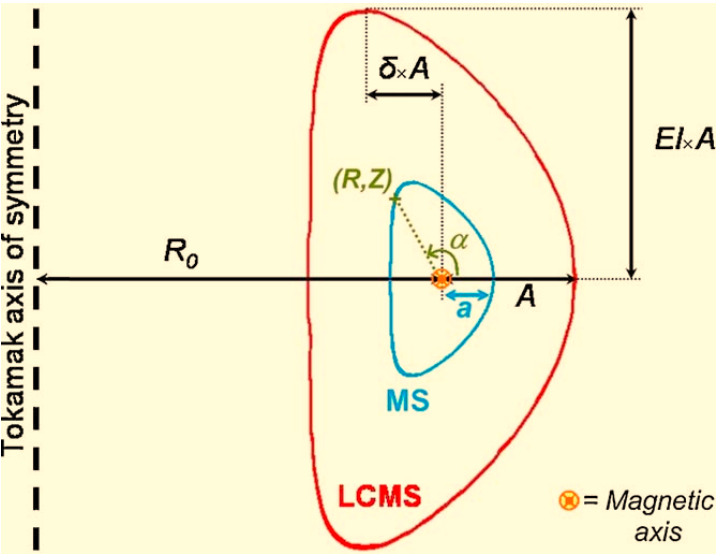
\includegraphics[scale=0.2]{../plots/Analytic_source.png}
  \caption{The analytic source configuration}
  \label{fig:Analytic_source}
\end{figure}

\section{Neutron Wall Loading} \label{Neutron Wall Loading}
The first step in the analysis applied to the full 3-D model involved calculations of the NWL distributions at the IB \& OB FWs, the inner \& outer divertor plates, and the middle divertor plate (dome). The vertical distribution of the NWL at the FWs (figure \ref{fig:NWL FWs}) and inner \& outer divertor plates (figure \ref{fig:NWL 2Divs}) were calculated over segments $\sim$ \SI{10}{cm} high. The radial distribution of the NWL at the dome is shown in figure \ref{fig:NWL Dome}. Table \ref{NWL peak and average values} shows the calculated peak and average values at the FWs and divertors. The peak values at the FWs occur at the midplane while for the inner and outer divertors it occurs at the bottom portion of the plate where it's closer to the plasma source. For the inner dome the peak value occurs at the middle.  
\begin{table}
	\caption{NWL peak and average values}
	\label{NWL peak and average values}
	\begin{tabular}{ |c|c|c|c| } 
		\hline
		 {} & Peak NWL [MW/m\textsuperscript{2}] & Average NWL [MW/m\textsuperscript{2}] \\
		\hline
		{OB FW} & 1.75 $\pm$ 0.11\% & 1.35 \\
		\hline
		{IB FW} & 1.31 $\pm$ 0.17\% & 0.86 \\
		\hline
		{Inner Divertor} & 0.79 $\pm$ 0.25\% & 0.32 \\
		\hline
		{Dome} & 0.66 $\pm$ 0.27\% & 0.49 \\
		\hline
		{Outer Divertor} & 0.76 $\pm$ 0.14\% & 0.35 \\
		\hline
		{3 Divertor plates} & 0.79 $\pm$ 0.13\% & 0.38 \\
		\hline
	\end{tabular}
\end{table}
 \begin{figure}[h!]
  \centering
  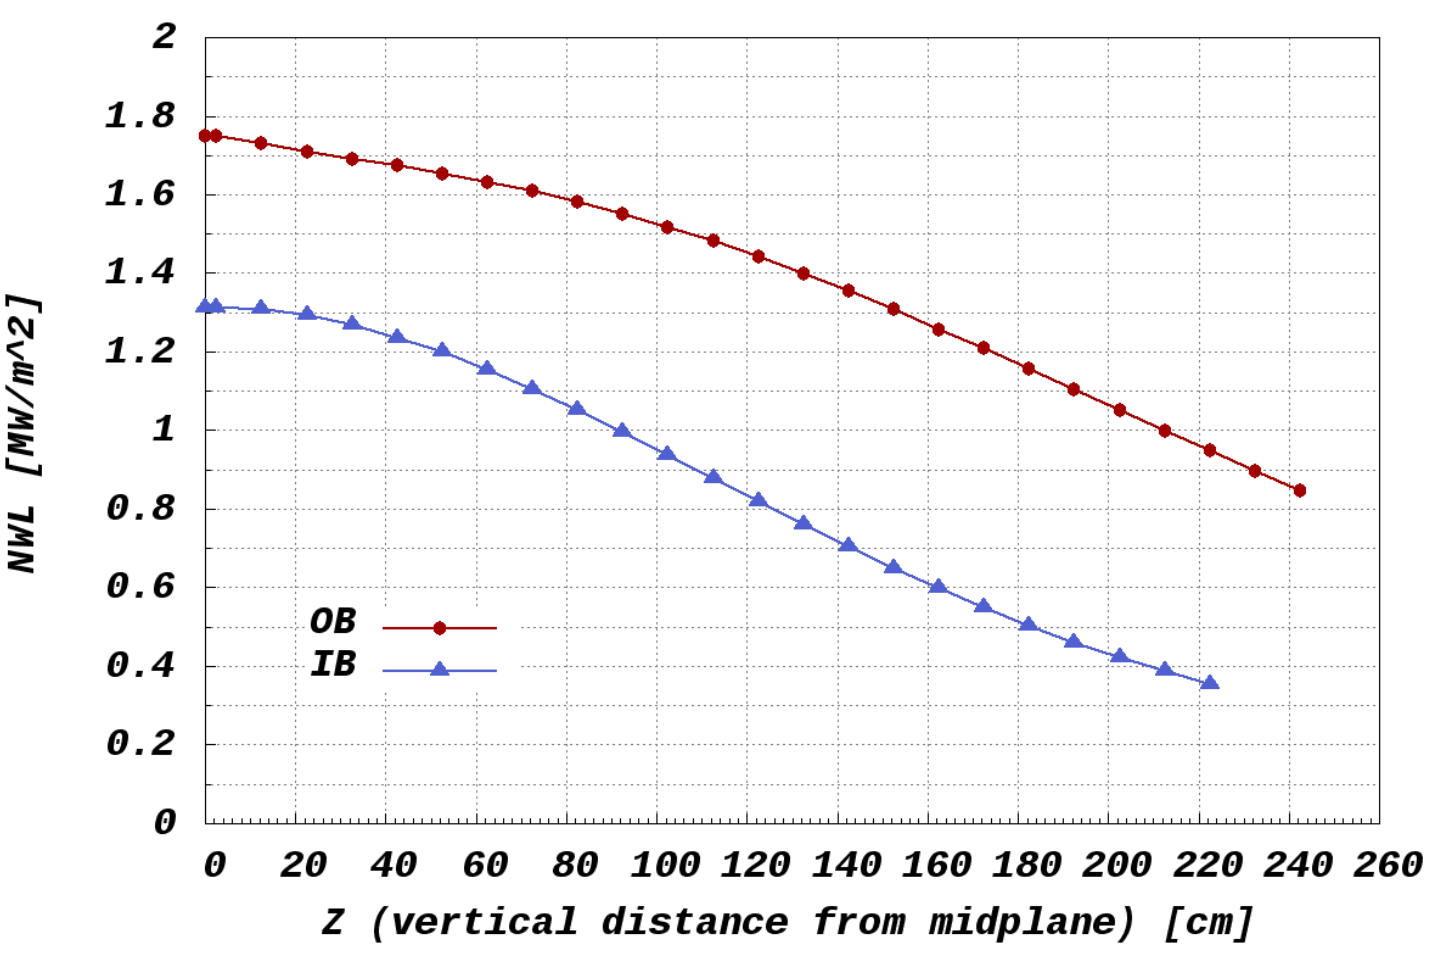
\includegraphics[scale=0.2]{../plots/NWL_FWs.png}
  \caption{The NWL vertical distribution at IB $\&$ OB FW}
  \label{fig:NWL FWs}
\end{figure}
\begin{figure}[h!]
  \centering
  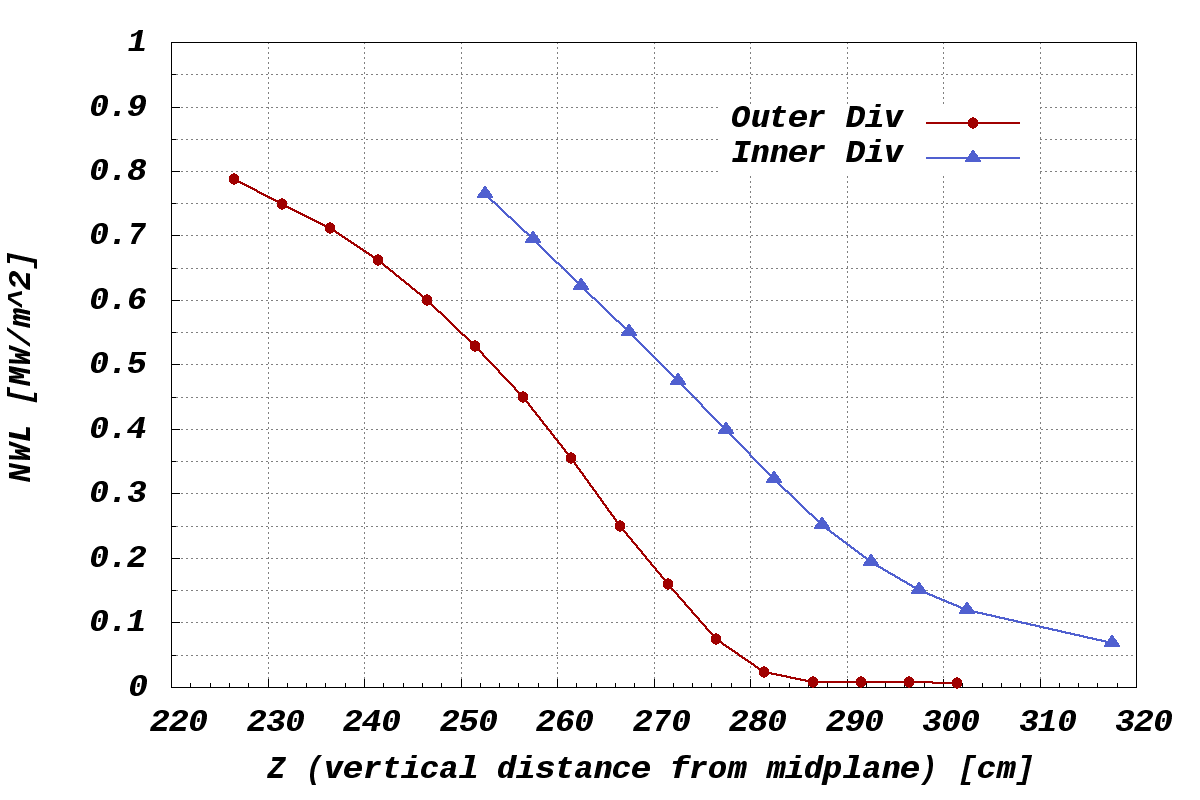
\includegraphics[scale=0.3]{../plots/NWL_2divs.png}
  \caption{The NWL vertical distribution at the inner and outer divertors}
  \label{fig:NWL 2Divs}
\end{figure}
\begin{figure}[h!]
	\centering
	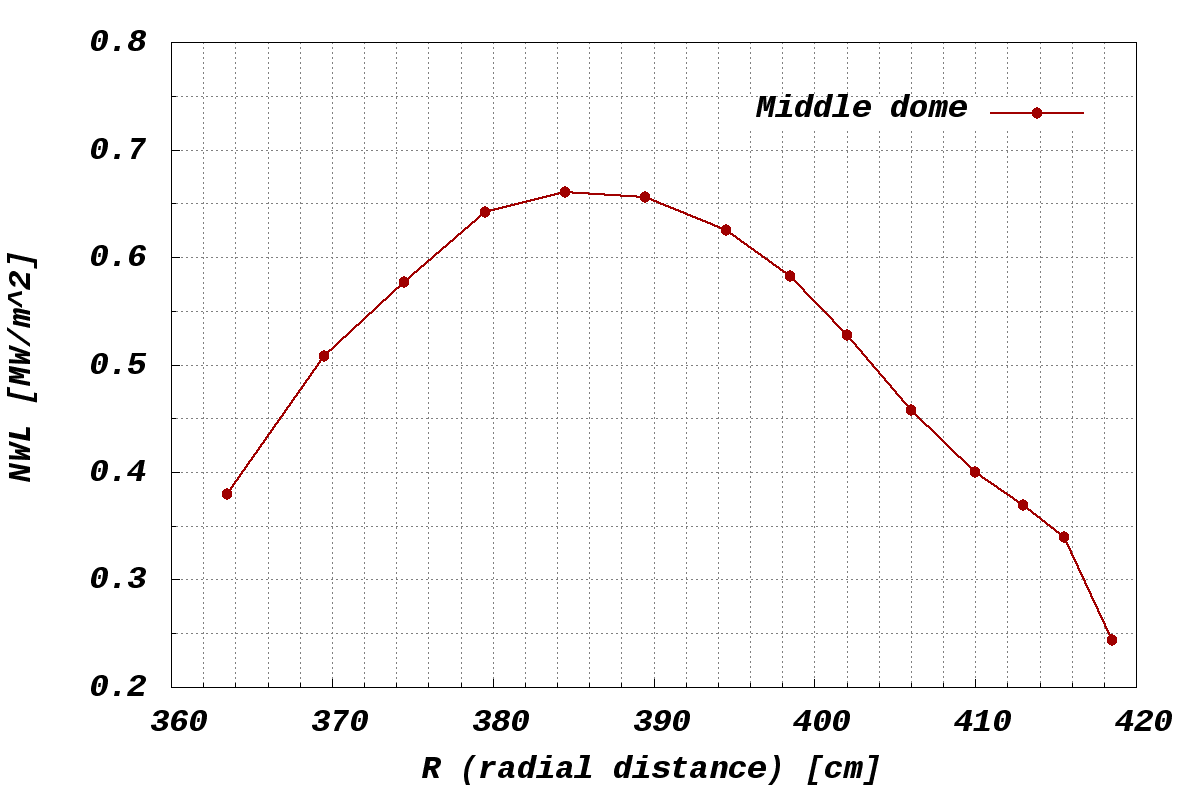
\includegraphics[scale=0.3]{../plots/NWL_div.png}
	\caption{The NWL distribution at the dome}
	\label{fig:NWL Dome}
\end{figure}

\section{Tritium Breeding Calculations} \label{Tritium Breeding Calculations}
The rich fusion research literature shows a growing interest to achieve ignition via the D-T fuel cycle and because of to the scarcity of T in nature and the high cost of T consumed by fusion power plants (55.6 kg/full power year (FPY)/GW) \cite{ref_4}, all power plants developed to date that employs the D-T fuel cycle are required to breed T in blankets surrounding the plasma. As a result the the need for TBR (ratio of tritium bred in the blankets to that consumed in the plasma) calculations with high certainty grew substantially and the TBR is considered an essential metric in the design phase.

The blanket of choice for the FESS-FNSF project is the dual cooled lead-lithium (DCLL) \cite{ref_8} blanket. The blanket consists of $\pm$ \SI{20}{cm} radial/toroidal flow channels of LiPb eutectic (15.7 at\% Li (90\% Li6 enrichment) and 84.3 at\% Pb) surrounded by \SI{0.5}{cm} SiC FCI (flow channel insert) and \SI{0.2}{cm} layer of LiPb. The blanket is cooled by helium at high pressure (\SI{8}{MPa}) which is also used for heat removal in other components such as FW and blanket side/back/front walls. The blanket also serves other purposes besides breeding T such as the removal of volumetric heat deposited by fast neutrons from the plasma and shielding the outer components; structural ring (SR), vacuum vessel (VV), and magnets.
\subsection{TBR Workflow} \label{TBR Workflow}
workflow steps
\subsection{Penetrations and Ports} \label{Penetrations and Ports}
figure and results
\subsection{Li-6 Enrichment} \label{Li-6 Enrichment}
One of the advantages of the DCLL blanket is allowing the control of the T bred by controlling the  Li6 enrichment in LiPb in the main flow channels. Controlling Li6 enrichment is necessary to avoid dealing with a surplus or shortage of T. Analyses were performed to test the effect of changing Li6 enrichment on the overall TBR of the facility (with all penetrations and ports included) and it was found that the TBR dropped to $1.0191\pm 0.03\%$, $0.9892\pm 0.03\%$, and $0.9513\pm 0.03\%$ for 70\%, 60\%, and 50\% Li6  enrichment, respectively. The TBR satisfies the tritium breeding requirement of 1.04 with ~ 80\% Li6 enrichment and the results are shown in figure 6.
\begin{figure}[h!]
  \centering
  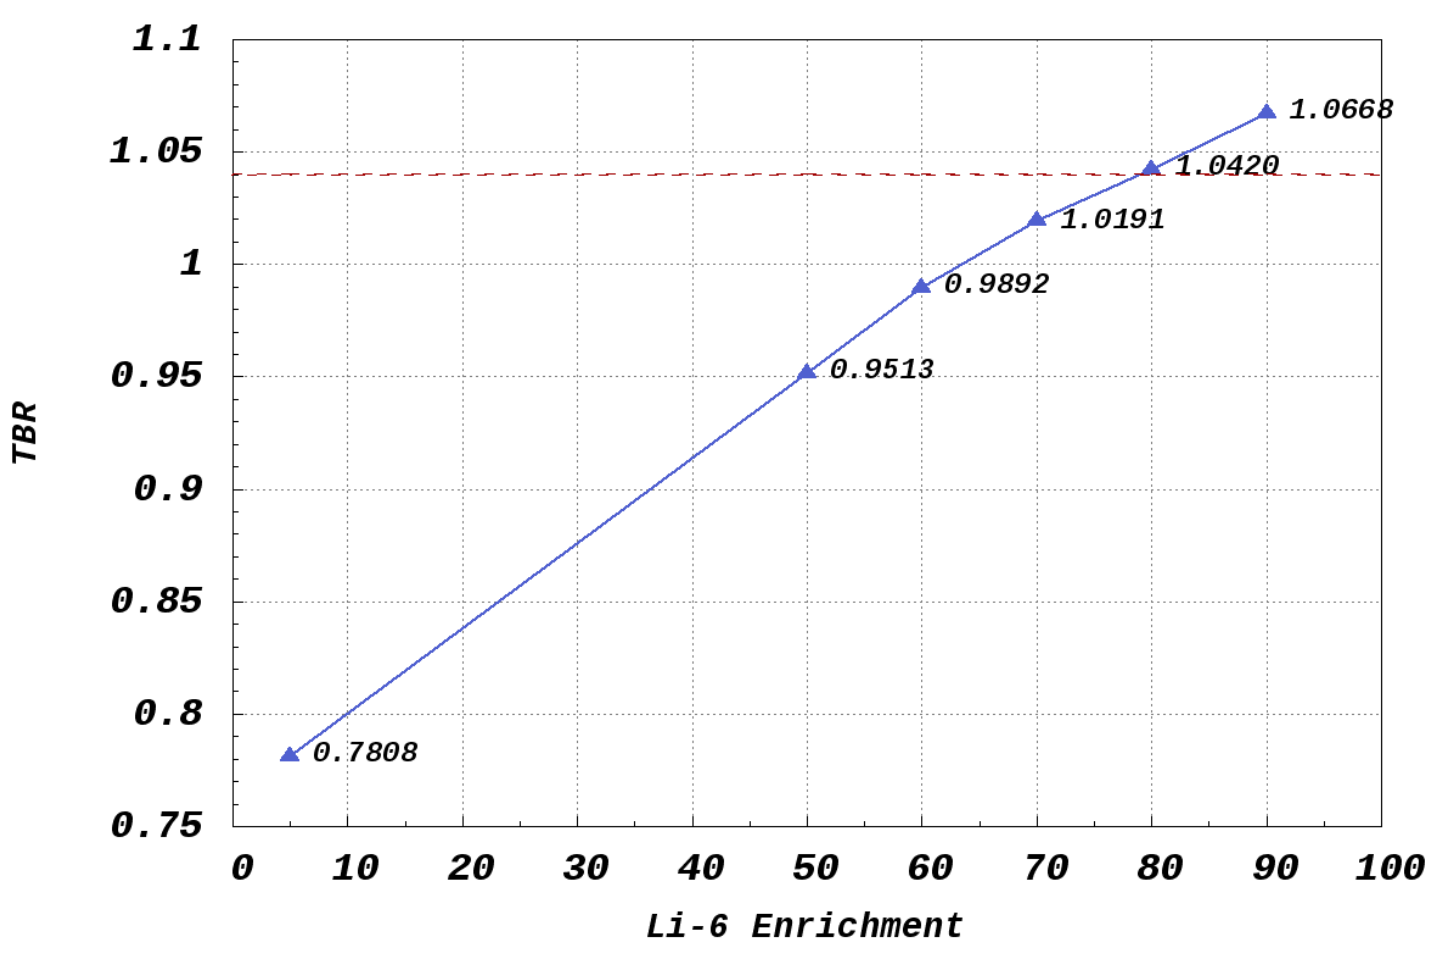
\includegraphics[scale=0.2]{../plots/Li6_enrichment.png}
  \caption{The facility overall TBR vs Li6 enrichment}
  \label{fig:Li6_enrichment}
\end{figure}
chart
\subsection{TBR mapping} \label{TBR mapping}
mapping of NBI, step 7, LH
importance of middle region

\section{Radiation Damage} \label{Radiation Damage}
\subsection{dpa, He/H production} \label{dpa, He/H production}
at FW and radial distribution of damage
\subsection{Magnet damage} \label{Magnet damage}
fast neutron fluence, heating, dpa to Cu stabilizer

\section{Shutdown Dose Rate Calculations} \label{Shutdown Dose Rate Calculations}
introduction and r2s worflow
\subsection{SDR} \label{SDR}
\subsection{Decay Heat} \label{Decay Heat}

\newpage
\section{References}
\begin{thebibliography}{10} 
\bibitem{ref_1} 
C. E. KESSEL, et al., {“The Fusion Nuclear Science Facility, the Critical Step in the Pathway to Fusion Energy,” Fusion Science and Technology, vol. 68, p. 225–236 (2015).}
\bibitem{ref_2} 
L. El-Guebaly, et al., {“Design Approach for FESS-FNSF In-Vessel Components and Constraints Imposed on Radial/Vertical Build Definition,” presented at 22nd ANS Topical Meeting on the Technology of Fusion Energy (TOFE), August 22 -25, 2016, Philadelphia, PA. To be published in Fusion Science and Technology.}
\bibitem{ref_3}
Clement Fausser, et al., {“Tokamak D-T Neutron Source Models for Different Plasma Physics Confinement Modes.” Fusion Engineering and Design, vol. 87, p. 787–792 (2012).} 
\bibitem{ref_4}
L. A. EL-GUEBALY, et al., {“Toward the Ultimate Goal of Tritium Self-Sufficiency: Technical Issues and Requirements Imposed on ARIES Advanced Power Plants,” Fusion Engineering and Design, vol. 84, p. 2072-2083 (2009).}
\bibitem{ref_5}
X-5 Monte Carlo Team, {MCNP a General Monte Carlo N-Particle Transport Code Version 5, Tech. Rep. LA-CP-03-0245, Los Alamos National Laboratory, MCNP 5, (March 2005).}
\bibitem{ref_6}
{DAGMC: http://svalinn.github.io/DAGMC/}
\bibitem{ref_7}
D. L. ALDAMA and et al., {“FENDL2.1, Update of an Evaluated Nuclear Data Library for Fusion applications.” IAEA report INDC (NDS) 467, Vienna, Austria (2004).}
\bibitem{ref_8}
S. MALANG et al., {“Development of the Lead Lithium (DCLL) Blanket Concept,” Fusion Science and Technology, 60, 249 (2011).}
\end{thebibliography}

\end{document}